\documentclass[english]{article}
\usepackage[T1]{fontenc}
\usepackage[latin9]{inputenc}
\usepackage{babel}

\usepackage{graphicx}
\usepackage[hidelinks]{hyperref}

% Use the PLoS provided bibtex style temporarily
\bibliographystyle{plos2009}

\begin{document}

\title{Making Data Count}


\author{John Kratz\textsuperscript{1{*}}, Carly Strasser\textsuperscript{1}}

\maketitle
1. California Digital Library 
{*}corresponding author(s): John Kratz (John.Kratz@ucop.edu)


\section*{Comment}

% ==============================================================
% Introduction
% ==============================================================

Data undergirds all of science and published data should be recognized as valuable scholarship, but scholarly recognition relies on accepted metrics of significance-- which data lacks.
The impact of a journal article has traditionally been estimated by counting the number of subsequent articles that cite it. 
A suite of internet-based alternative metrics (``altmetrics'') seek to provide faster assessment and to capture other kinds of impact \cite{priem_altmetrics_2012}.
Article-centered metrics like these can measure data by proxy, via data descriptor articles in journals like \textit{Earth Systems Science Data} or \textit{Scientific Data}\cite{pfeiffenberger_earth_2011, editors_more_2014}.
Or, article metrics can be applied to datasets themselves.
However, the translation is not always straightforward; opening a web page, downloading, or citing all mean different things if the target is a dataset rather than an article.

Several groups are investigating traditional, alternative, and novel metrics for data. 
The Research Data Alliance Data Bibliometrics Working Group aims to ``conceptualize data metrics and corresponding services'' (\url{http://rd-alliance.org/group/rdawds-publishing-data-bibliometrics-wg/case-statement/rdawds-publishing-data-bibliometrics-wg}{}). 
The National Information Standards Organization (NISO) Alternative Assessment Metrics Initiative explicitly includes non-traditional products like software and data (\url{http://www.niso.org/topics/tl/altmetrics_initiative/}).  
Here, we present results from Making Data Count (\url{http://mdc.plos.org}), a collaboration between the California Digital Library, the Public Library of Science (PLOS), and DataONE to define a suite of data metrics, then adapt the existing PLOS Article Level Metric tool (\url{http://alm.plos.org}) to capture and present them.


% ==============================================================
% Methods and Demographics
% ==============================================================

To develop useful metrics, we must understand the needs and values of both the researchers who create and use data, and the data managers who preserve and publish it.
Before Making Data Count was conceived, we had conducted a survey of researcher perspectives on data publication that touched briefly on metrics of impact; respondents to that survey found citation and download counts much more useful than search rank or altmetrics \cite{kratz_researcher_2015}.
During the research phase of Making Data Count, we expanded on this work with new surveys for researchers and data managers about data sharing, discovery, and metrics.
In November and December of 2014, we solicited responses to a pair of online surveys via social media, listservs, and posts to CDL and PLOS blogs-- ultimately hearing from 247 researchers and 73 data managers \cite{kratz_making_2015}.
Most researchers worked at academic institutions (78\%), and most were based in the United States (57\%) or United Kingdom (14\%).
Both academic (64\%) and government-run (22\%) repositories were significantly represented; repositories were primarily located in the United States (72\%) or United Kingdom (11\%).
Researcher respondents covered the academic career spectrum, from principal investigators (42\%), to postdocs (21\%), and graduate students (19\%). 
Biology was the best-represented discipline (53\%), along with environmental (17\%) and social (10\%) science. 


% ==============================================================
% Locations for sharing
% ==============================================================

To collect and communicate data metrics, we need to know where on the internet researchers go to share their data or to search for data to use. 
Fortunately, data sharing behavior has been well-studied \cite{tenopir_data_2011, akers_disciplinary_2013, wallis_if_2013, aydinoglu_data_2014, kratz_researcher_2015}. 
Consistent with previous surveys, direct transmission (e.g., via email) on request was the most common behavior: 74\% of respondents had shared some data and 16\% had shared ``most/all'' of their data that way.
Among the drawbacks to this approach-- including the potential for capricious denial of access-- is that it is invisible to measurement. 
Fortunately, researchers also often share over a more tractable channel: 71\% have published data in a database or repository.
The researchers who shared the most were especially likely to do so that way; 57\% of the 94 respondents who shared most/all of their data put it in a database or repository.


% ==============================================================
% Information about data users
% ==============================================================

Researchers want to know who is using their data for what purpose \cite{tenopir_data_2011, bobrow_establishing_2014}.
This understandable wish explains, in part, the popularity of sharing on request.
Public repositories could satisfy this interest by presenting metrics of data users, while making the data more readily available.
We asked researchers to rank their interest in five pieces of information about users of their data; not surprisingly, the most detailed option was also the most popular.
Almost half (48\%) ranked ``name and contact information,''  as the most interesting, many fewer chose the less-specific options: discipline (32\%), institution type (8\%), institutional affiliation (6\%), and geographic location (5\%).
However, a substantial proportion (13\%) ranked this option last, and average interest in discipline was equally high.
When asked a similar question, 67\% of data managers were most interested in discipline.
Half of the repositories collect extensive information-- a name (47\%), email address (44\%), and institutional affiliation (40\%)-- and half (47\%) do not collect any.


% ==============================================================
% Discovery & use
% ==============================================================

Relative to data sharing, where and how researchers search for data to (re-)use is poorly understood.
We asked researchers how likely they would be to use each of five strategies (shown in Figure \ref{fig:results}a); no single method predominated.
Three different strategies would definitely be used by most respondents: searching via references in the literature (59\%), a discipline-specific database (58\%), or a general purpose search engine (51\%). 
Taken together, 63\% of respondents would ``definitely'' employ two or more strategies.
When we asked respondents to write-in particular sources, they most frequently ($n=16$) mentioned the general-purpose repository Dryad (\url{http://datadryad.org/}); Google and ``journal articles'' tied for second ($n=14$). 
Respondents generally did not `crowd-source' data discovery via open inquiries on social media (42\% ``no chance'') or discussion forums (40\% no chance).
However, direct inquiries (by email or in person) to knowledgeable colleagues are probably common, and were a frequent ($n=12$) write-in discovery source.

We next sought to characterize how our respondents use public data once they have found it.
We asked how frequently they used public data early (to generate ideas/hypotheses), as the central piece (to reach the main conclusion), or late (to support the main conclusion) in their research process (Figure \ref{fig:results}b).
An overwhelming 96\% of respondents at least ``occasionally'' use public data, and a 56\% majority used public data ``often.''
Furthermore, although use early (41\% often, 46\% occasionally) and late (39\% often, 47\% occasionally) were higher, much of this use is central to research-- 28\% often and 42\% occasionally use public data to reach central conclusions.


% ==============================================================
% Data impact 
% ==============================================================

Among the potential audiences for data metrics-- administrators, funders, data managers-- the most invested are undoubtedly dataset creators.
In addition to providing researchers with a sense of what their data is being used for, metrics can reassure them that it is actually being used and that the effort to share it was not wasted.
Secondarily, data managers have a stake in knowing about use of their data to tailor services and justify funding. 
To learn about the immediate interests of these groups, we asked them to rank several potential metrics of impact. 

Both groups measure scholarly prestige in citations: 85\% of researchers (Figure \ref{fig:results}c) and 61\% of data managers ranked citations as the most interesting metric. 
In the case of researchers, this preference is consistent with our earlier survey \cite{kratz_researcher_2015}.
Most researchers (64\%) ranked downloads second. 
Majorities of both researchers and data managers ranked landing page views last.

For practical reasons, we can not implement data metrics without understanding what metrics of data use repositories collect (Figure \ref{fig:results}d). 
Most repositories track downloads (85\%) and landing page views (66\%). 
But, only 30\% display download counts (and 27\% page views) on the landing page or provide them through a program interface.
A 2013 survey of 35 repositories arrived at a similar figure: 20\% of those displayed dataset level metrics \cite{costas_value_2013}.
Across the board, the metrics in our survey were displayed by only one-third of the repositories that track them.
Despite high interest in citation counts, relatively few repositories (23\%) track them, presumably because this is much more challenging. 

% ==============================================================
% Conclusions & future work 
% ==============================================================

Citations are the coin of the academic realm, but their present usefulness for data is limited because datasets are rarely cited formally \cite{robinson-garcia_analyzing_2015}.
A 2011 survey of social science papers best illuminates current practice: only 17\% of papers that used published data cited it in the reference list, roughly the same percentage as in 1995 \cite{sieber_not_1995, mooney_citing_2011}. 
However, we do believe that the situation will improve. 
Researchers strongly favor formal data citation.
In a cross-disciplinary 2011 survey, 95\% of respondents agreed that formal citation is a fair condition for data sharing, as did 87\% of astrobiologists in a follow-up survey \cite{tenopir_data_2011, aydinoglu_data_2014}. 
Citation ``in the references like normal publications'' is the preferred method of receiving credit for data sharing by 71\% of biodiversity researchers and by 75\% of respondents to our earlier survey \cite{enke_users_2012, kratz_researcher_2015}.
In 2014, the scholarly communication community arrived at a Joint Declaration of Data Citation Principles (\url{http://www.force11.org/node/4769}) with formal citation at its core. 
The Joint Declaration has since been endorsed by 91 repositories, publishers, and scholarly organizations-- including DataCite, the Research Data Alliance, and Nature Publishing Group (\url{http://blogs.nature.com/scientificdata/2014/03/24/endorsing-the-joint-declaration-of-data-citation-principles/}).
\emph{Scientific Data} data descriptors, for example, are formatted in accordance with the Joint Declaration, and each includes at least one formal data citation.

In contrast to citations, repositories can easily track data landing page views and downloads today.
Page views are of little value to researchers or data managers, but downloads are more highly regarded.
(It stands to reason that downloading a dataset represents a higher level of engagement that viewing a landing page.)
Researchers consistently ranked downloads as their second-choice metric.
Our previous survey suggests that, the gap in perceived value between citations and downloads is surprisingly narrow \cite{kratz_researcher_2015}.
Most repositories already track downloads, and we strongly recommend that more of them make download counts public.

This survey provides several clear points of guidance for Making Data Count and anyone invested in data metrics.
In the short-term, page views and social media activity can be deemphasized because of low status and lack of data-related activity respectively.
While challenging, citations should be emphasized and collected as best as possible.
One approach that we are taking in Making Data Count is to search the full text of PLOS articles for informally cited datasets.
Downloads should be emphasized as, at present, a happy medium: both reasonably valuable and reasonably easy to measure.
While we would be pleased to see more sophisticated schemes to apportion scholarly credit and facilitate knowledge discovery \cite{ingwersen_indicators_2011, ding_enititymetrics_2013, katz_transitive_2014} catch on, these straightforward metrics fulfill an immediate need to quantify data impact in a way that all of the stakeholders-- including data managers, administrators, and researchers-- can understand today.


\section*{Acknowledgements}

Making Data Count is funded by National Science Foundation (NSF) grant number 1448821.


\section*{Competing financial interests}


The author(s) declare no competing financial interests.


\section*{Figures Legends}

% Figure should be referred to using a consistent numbering scheme through
% the entire Data Descriptor. For initial submissions, authors may choose
% to supply this document as a single PDF with embedded figures, but
% separate figure image files must be provided for revisions and accepted
% manuscripts. In most cases, a Data Descriptor should not contain more
% than three figures, but more may be allowed when needed. We discourage
% the inclusion of figures in the Supplementary Information \textendash{}
% all key figures should be included here in the main Figure section. 

% Figure legends begin with a brief title sentence for the whole figure
% and continue with a short description of what is shown in each panel,
% as well as explaining any symbols used. Legend must total no more
% than 350 words, and may contain literature references. 

\begin{figure}[!ht]
\begin{center}
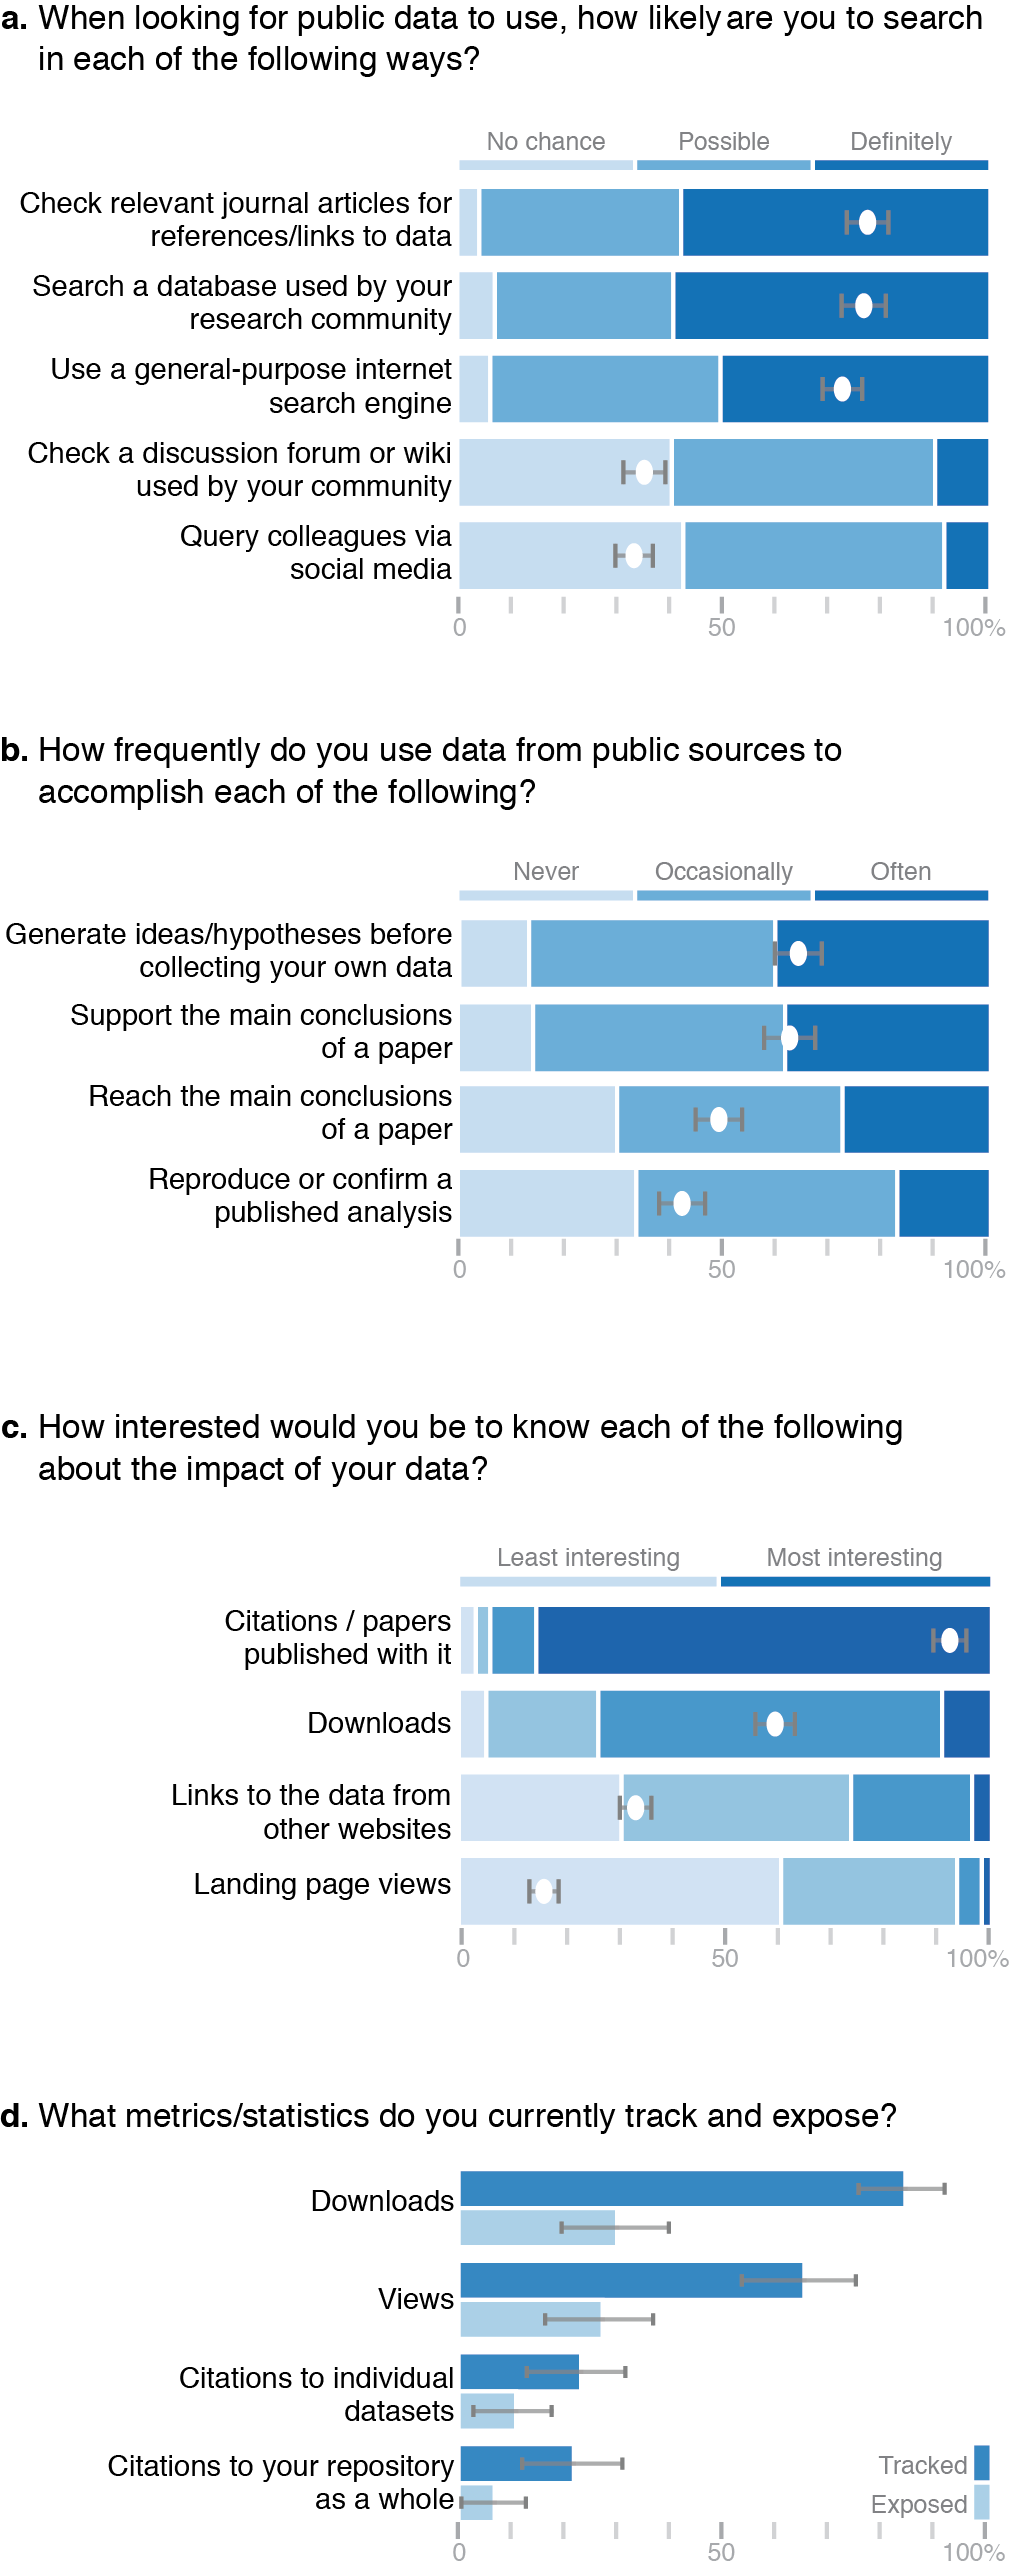
\includegraphics[width=3.25in]{MDC_Figure.png}
\end{center}
\caption{
{\bf Researchers value citations and download counts; most repositories track downloads but few expose them.}
Researchers ($n=247$) indicated (a.) how they search for data and (b.) how they subsequently use it; and (c.) ranked their relative interest in four possible metrics of impact.
Data managers ($n=71$) (d.) reported which of metrics their repositories track and expose.
White dots show the mean on a scale of 1-3 (a. and b.) or 1-4 (c.).
All error bars depict 95\% confidence intervals calculated by basic bootstrap with 10,000 resamplings. 
}
\label{fig:results}
\end{figure}

\begin{thebibliography}{10}
\providecommand{\url}[1]{\texttt{#1}}
\providecommand{\urlprefix}{URL }
\expandafter\ifx\csname urlstyle\endcsname\relax
  \providecommand{\doi}[1]{doi:\discretionary{}{}{}#1}\else
  \providecommand{\doi}{doi:\discretionary{}{}{}\begingroup
  \urlstyle{rm}\Url}\fi
\providecommand{\bibAnnoteFile}[1]{%
  \IfFileExists{#1}{\begin{quotation}\noindent\textsc{Key:} #1\\
  \textsc{Annotation:}\ \input{#1}\end{quotation}}{}}
\providecommand{\bibAnnote}[2]{%
  \begin{quotation}\noindent\textsc{Key:} #1\\
  \textsc{Annotation:}\ #2\end{quotation}}
\providecommand{\eprint}[2][]{\url{#2}}

\bibitem{priem_altmetrics_2012}
Priem J, Piwowar HA, Hemminger BM (2012) Altmetrics in the wild: {Using} social
  media to explore scholarly impact.
\newblock {arXiv} e-print 1203.4745.
\newblock \urlprefix\url{http://arxiv.org/abs/1203.4745}.
\bibAnnoteFile{priem_altmetrics_2012}

\bibitem{pfeiffenberger_earth_2011}
Pfeiffenberger H, Carlson D (2011) "{Earth} {System} {Science} {Data}" ({ESSD})
  — {A} {Peer} {Reviewed} {Journal} for {Publication} of {Data}.
\newblock D-Lib Magazine 17.
\bibAnnoteFile{pfeiffenberger_earth_2011}

\bibitem{editors_more_2014}
{Editors} (2014) More bang for your byte.
\newblock Scientific Data 1.
\bibAnnoteFile{editors_more_2014}

\bibitem{kratz_researcher_2015}
Kratz JE, Strasser C (2015) Researcher {Perspectives} on {Publication} and
  {Peer} {Review} of {Data}.
\newblock PLoS ONE 10: e0117619.
\bibAnnoteFile{kratz_researcher_2015}

\bibitem{kratz_making_2015}
Kratz JE, Strasser C (2015) Making {Data} {Count} survey responses.
\newblock University of California, Office of the President .
\bibAnnoteFile{kratz_making_2015}

\bibitem{tenopir_data_2011}
Tenopir C, Allard S, Douglass K, Aydinoglu AU, Wu L, et~al. (2011) Data
  {Sharing} by {Scientists}: {Practices} and {Perceptions}.
\newblock PLoS ONE 6: e21101.
\bibAnnoteFile{tenopir_data_2011}

\bibitem{akers_disciplinary_2013}
Akers KG, Doty J (2013) Disciplinary differences in faculty research data
  management practices and perspectives.
\newblock International Journal of Digital Curation 8: 5--26.
\bibAnnoteFile{akers_disciplinary_2013}

\bibitem{wallis_if_2013}
Wallis JC, Rolando E, Borgman CL (2013) If {We} {Share} {Data}, {Will} {Anyone}
  {Use} {Them}? {Data} {Sharing} and {Reuse} in the {Long} {Tail} of {Science}
  and {Technology}.
\newblock PLoS ONE 8: e67332.
\bibAnnoteFile{wallis_if_2013}

\bibitem{aydinoglu_data_2014}
Aydinoglu AU, Suomela T, Malone J (2014) Data {Management} in {Astrobiology}:
  {Challenges} and {Opportunities} for an {Interdisciplinary} {Community}.
\newblock Astrobiology 14: 451--461.
\bibAnnoteFile{aydinoglu_data_2014}

\bibitem{bobrow_establishing_2014}
Bobrow M, Banks J, Burton P, Smith GD, Eeles R, et~al. (2014) Establishing
  {Incentives} and {Changing} {Cultures} to {Support} {Data} {Access}.
\newblock Technical report, Wellcome Trust.
\newblock
  \urlprefix\url{http://www.wellcome.ac.uk/stellent/groups/corporatesite/@msh_peda/documents/web_document/wtp056495.pdf}.
\newblock Expert Advisory Group on Data Access.
\bibAnnoteFile{bobrow_establishing_2014}

\bibitem{costas_value_2013}
Costas R, Meijer I, Zahedi Z, Wouters P (2013) The {Value} of {Research} {Data}
  {Metrics} for datasets from a cultural and technical point of view.
\newblock Technical report.
\newblock \urlprefix\url{http://www.knowledge-exchange.info/datametrics}.
\bibAnnoteFile{costas_value_2013}

\bibitem{robinson-garcia_analyzing_2015}
Robinson-Garcia N, Jiménez-Contreras E, Torres-Salinas D (2015) Analyzing data
  citation practices according to the {Data} {Citation} {Index}.
\newblock arXiv:150106285 [cs] .
\bibAnnoteFile{robinson-garcia_analyzing_2015}

\bibitem{sieber_not_1995}
Sieber PJE, Trumbo BE (1995) ({Not}) giving credit where credit is due:
  {Citation} of data sets.
\newblock Science and Engineering Ethics 1: 11--20.
\bibAnnoteFile{sieber_not_1995}

\bibitem{mooney_citing_2011}
Mooney H (2011) Citing data sources in the social sciences: do authors do it?
\newblock Learned Publishing 24: 99--108.
\bibAnnoteFile{mooney_citing_2011}

\bibitem{enke_users_2012}
Enke N, Thessen A, Bach K, Bendix J, Seeger B, et~al. (2012) The user's view on
  biodiversity data sharing — {Investigating} facts of acceptance and
  requirements to realize a sustainable use of research data —.
\newblock Ecological Informatics 11: 25--33.
\bibAnnoteFile{enke_users_2012}

\bibitem{ingwersen_indicators_2011}
Ingwersen P, Chavan V (2011) Indicators for the {Data} {Usage} {Index} ({DUI}):
  an incentive for publishing primary biodiversity data through global
  information infrastructure.
\newblock BMC Bioinformatics 12: S3.
\bibAnnoteFile{ingwersen_indicators_2011}

\bibitem{katz_transitive_2014}
Katz DS (2014) Transitive {Credit} as a {Means} to {Address} {Social} and
  {Technological} {Concerns} {Stemming} from {Citation} and {Attribution} of
  {Digital} {Products}.
\newblock Journal of Open Research Software 2: e20.
\bibAnnoteFile{katz_transitive_2014}

\end{thebibliography}



\end{document}

